\documentclass[10pt]{article}

\usepackage[T1]{fontenc}
\usepackage[utf8]{inputenc}
\usepackage{newtxtext,newtxmath}
\usepackage[final]{microtype}
\usepackage[letterpaper,margin=0.86in,headheight=14pt]{geometry}
\usepackage{amsmath,bm}
\usepackage{booktabs,tabularx,longtable,array}
\usepackage{float}
\usepackage{enumitem}
\usepackage{xcolor}
\usepackage{tikz}
\usetikzlibrary{arrows.meta,positioning}
\usepackage{listings}
\usepackage{xurl}
\usepackage{hyperref}
\usepackage[nameinlink,capitalise,noabbrev]{cleveref}
\usepackage{fancyhdr}
\usepackage{titlesec}
\usepackage{caption}
\usepackage{siunitx}

\definecolor{navy}{HTML}{17365D}
\definecolor{blue}{HTML}{2E75B6}
\definecolor{lightblue}{HTML}{EAF2F8}
\definecolor{darkgray}{HTML}{3F4650}
\definecolor{lightgray}{HTML}{F3F4F6}
\definecolor{darkgreen}{HTML}{2F6B4F}
\definecolor{darkred}{HTML}{9C2F2F}

\hypersetup{
  colorlinks=true,
  linkcolor=navy,
  citecolor=darkgreen,
  urlcolor=blue,
  pdftitle={Optimizing RBF SVM Training on Modern GPUs},
  pdfauthor={Jiang Yongchun},
  pdfsubject={Technical report on GPU kernel SVM optimization},
  pdfkeywords={support vector machine, SMO, GPU, CUDA, low precision, kernel cache}
}

\sisetup{detect-all,group-digits=integer,group-separator={,}}
\setlist[itemize]{leftmargin=1.45em,itemsep=2pt,topsep=3pt}
\setlist[enumerate]{leftmargin=1.65em,itemsep=2pt,topsep=3pt}
\renewcommand{\arraystretch}{1.12}

\newcolumntype{Y}{>{\raggedright\arraybackslash}X}
\newcolumntype{L}[1]{>{\raggedright\arraybackslash}p{#1}}
\newcommand{\code}[1]{\texttt{#1}}
\newcommand{\researchq}[1]{\textbf{RQ#1}}

\pagestyle{fancy}
\fancyhf{}
\fancyhead[L]{\small GPU RBF SVM Training}
\fancyhead[R]{\small Technical Report TR-SVM-2026-07-27}
\fancyfoot[C]{\thepage}
\renewcommand{\headrulewidth}{0.35pt}

\titleformat{\section}
  {\large\bfseries\color{navy}}{\thesection}{0.65em}{}
\titleformat{\subsection}
  {\normalsize\bfseries\color{darkgray}}{\thesubsection}{0.6em}{}
\titleformat{\subsubsection}
  {\normalsize\bfseries}{\thesubsubsection}{0.55em}{}
\titlespacing*{\section}{0pt}{1.35em}{0.55em}
\titlespacing*{\subsection}{0pt}{1.0em}{0.35em}

\captionsetup{font=small,labelfont=bf}

\lstdefinestyle{codeblock}{
  basicstyle=\ttfamily\small,
  backgroundcolor=\color{lightgray},
  frame=single,
  rulecolor=\color{lightgray},
  breaklines=true,
  columns=fullflexible,
  keepspaces=true,
  aboveskip=6pt,
  belowskip=6pt
}

\begin{document}

\hypersetup{pageanchor=false}
\begin{titlepage}
  \centering
  \vspace*{1.0in}
  {\Large\bfseries\color{navy}
    Optimizing RBF SVM Training on Modern GPUs\par}
  \vspace{0.22in}
  {\large Coherent Low Precision, Kernel Reuse, and the Limits of Parallel SMO\par}
  \vspace{0.55in}
  {\large Jiang Yongchun\par}
  \vspace{0.12in}
  {\normalsize Technical Report TR-SVM-2026-07-27\par}
  \vspace{0.08in}
  {\normalsize July 27, 2026\par}

  \vfill
  \begin{minipage}{0.88\textwidth}
    \small
    \noindent\textbf{Status.}
    This mechanism-centered public report studies how representation
    coherence, kernel-data reuse, and optimization dependency depth interact
    in GPU RBF SVM training. Measurements are reported with explicit workload
    and numerical boundaries. Private engineering provenance, superseded
    experiment logs, and implementation-specific development history are
    intentionally excluded.
  \end{minipage}
  \vspace{0.55in}
\end{titlepage}
\hypersetup{pageanchor=true}
\pagenumbering{roman}

\begin{abstract}
Training a nonlinear support vector machine (SVM) at scale is expensive
because decomposition solvers repeatedly generate kernel columns, update a
global gradient state, and execute a sequential working-set optimizer. This
report studies these costs on an NVIDIA RTX PRO 6000 Blackwell GPU using the
RBF C-SVC implementation in cuML 26.06 as the starting point. We redesign
kernel generation and reuse, then introduce a \emph{coherent-FP16} execution
path in which the persistent kernel cache and the local SMO subproblem consume
the same low-precision kernel representation. On EMBER-65K, coherent FP16
reduces median fit time from \SI{0.486954}{s} to \SI{0.360385}{s} relative to a
same-framework, equal-column-capacity direct FP32-cache control, a
\textbf{1.351$\times$} speedup over seven balanced fresh-process runs (95\%
bootstrap confidence interval: 1.263$\times$--1.403$\times$). The comparison
holds logical cache capacity fixed, not cache bytes. On all 200,000 official
EMBER test samples, a separately matched stock-model comparison changes
accuracy from 0.830980 to 0.830895 and ROC AUC from 0.93525055 to 0.93516107;
McNemar's test detects no statistically significant accuracy difference in
this experiment ($p=0.231645$). The coherent implementation does not satisfy
the original FP32-kernel KKT audit and must not be described as an exact FP32
drop-in solver.

After kernel acceleration, the serial SMO block solver becomes the dominant
GPU kernel, accounting for 40.3\% of the measured steady solver phase. We
evaluate whole-working-set projected and Newton methods, fixed-depth block-QP
updates, sampled candidate selection, geometry-aware pair packing,
stale-candidate prediction, exact-pair replay, triangular batching, and
speculative overlap. Real working-set captures and a 2,896-step exact GPU
trace show that these methods either introduce excessive dependent solves,
consume additional local kernel rows, increase global kernel-column work, or
retain a substantial serial step-and-update floor. The strongest
decision-path-aware block-solver micro-optimization provides only a
1.0376$\times$ paired geometric-mean end-to-end speedup. The resulting design
boundary is a work-depth constraint: a successful parallel SMO mechanism must
increase optimization progress per kernel data item while reducing dependent
stages and outer full-data scans.
\end{abstract}

\tableofcontents
\clearpage
\pagenumbering{arabic}

\section{Introduction}

Nonlinear kernel SVMs expose a form of GPU workload that is easy to
misdiagnose. Their expensive RBF evaluations resemble dense linear algebra,
but training is not a sequence of independent matrix multiplications. A
decomposition solver repeatedly selects a working set, produces or reuses
kernel data, solves a box-constrained local quadratic program, updates a
global gradient, and uses the new state to make the next decision. The
performance of the system is therefore determined jointly by regular numeric
work and a state-dependent optimization trajectory.

This distinction becomes more important as the regular work is accelerated.
Tensor Cores make batches of dot products inexpensive, compact kernel values
increase cache coverage, and fused kernels reduce intermediate traffic. These
optimizations can expose a different limit: pairwise sequential minimal
optimization (SMO) commits one update before the next pair can be selected.
At that point, low occupancy is not itself the problem. It is evidence that
the algorithm has little independent work to schedule. Increasing occupancy
by speculating, batching, or replaying updates is useful only if the extra
work produces enough optimization progress.

We use RBF SVM training to study this interaction between representation,
data reuse, and dependency depth. Four observations organize the study.
First, precision is a property of the complete state transition, not of one
GEMM or cache in isolation: all producers and decision-making consumers of a
kernel value must observe a coherent representation. Second, global kernel
columns, local working-set rows, and dependent solver stages have different
costs and cannot be summarized by FLOP/s or occupancy. Third, the relevant
unit of efficiency is the optimization progress obtained from each expensive
piece of kernel data, rather than the number of pair updates executed. Fourth,
the profitable mechanism changes with feature dimension and training phase,
so a single static kernel is unlikely to be uniformly optimal.

These observations lead to three research questions.

\begin{itemize}
  \item \researchq{1}: How do kernel generation, reuse, and local optimization
        interact to determine end-to-end GPU SVM performance?
  \item \researchq{2}: Can a coherent low-precision kernel representation
        improve end-to-end time while retaining measured predictive quality?
  \item \researchq{3}: When does reducing the dependency depth of pair-SMO
        improve time to convergence, rather than merely moving work into
        additional kernel rows, columns, or dense solves?
\end{itemize}

The study makes four contributions. First, it introduces a cost decomposition
that separates full-data kernel-column misses, local-row consumption, and
dependent decision stages. This decomposition explains why superficially
similar ``kernel scans'' can differ by orders of magnitude. Second, it
develops coherent-FP16 execution, in which cached kernel values and the local
solver use the same rounded operator. On EMBER-65K, this design is
1.351$\times$ faster than a direct-FP32-cache control over seven balanced
fresh-process runs. Third, it characterizes the resulting bottleneck
migration: after kernel representation and reuse improve, the dependent local
solver becomes the largest measured GPU kernel. Fourth, it evaluates several
ways to shorten that chain and shows why reducing apparent depth is
insufficient when it increases kernel-data work or outer iterations.

The claims are intentionally bounded. The 1.351$\times$ result is a matched
comparison on one high-dimensional workload, with equal logical cache
capacity rather than equal cache bytes. A separate held-out evaluation finds
no statistically significant accuracy difference between the saved stock
FP32 and coherent-FP16 models in that experiment, but it does not establish
cross-workload equivalence. Coherent FP16 also does not satisfy the original
FP32-kernel KKT audit and is therefore a distinct low-precision optimization
contract, not an exact FP32 replacement. The solver experiments establish
boundaries for the measured designs; they do not preclude a parallel SVM
solver that discovers more productive optimization directions.

\section{Background and Problem Formulation}

\subsection{RBF C-SVC dual}

For labels $y_i\in\{-1,+1\}$, the binary C-SVC dual is
\begin{equation}
  \min_{\bm{\alpha}}
  \quad
  \frac{1}{2}\bm{\alpha}^{\mathsf T}Q\bm{\alpha}
  -\bm{1}^{\mathsf T}\bm{\alpha},
  \label{eq:dual}
\end{equation}
subject to
\begin{equation}
  \bm{y}^{\mathsf T}\bm{\alpha}=0,
  \qquad
  0\leq \alpha_i\leq C.
  \label{eq:dual-constraints}
\end{equation}
The matrix entries are
\begin{equation}
  Q_{ij}=y_i y_j K(\bm{x}_i,\bm{x}_j),
  \qquad
  K(\bm{x}_i,\bm{x}_j)
  =\exp\!\left(-\gamma\lVert\bm{x}_i-\bm{x}_j\rVert_2^2\right).
  \label{eq:rbf}
\end{equation}
Materializing $Q\in\mathbb{R}^{N\times N}$ is prohibitive at scale.
Decomposition methods therefore optimize a working set while holding all
other variables fixed. SMO is the limiting two-variable method and uses an
analytic box-constrained update~\cite{platt1999smo}; second-order working-set
selection improves progress per step~\cite{fan2005working}.

\subsection{Execution pipeline}

The measured cuML path follows the five-stage pipeline in
\cref{fig:pipeline}.

\begin{figure}[t]
  \centering
  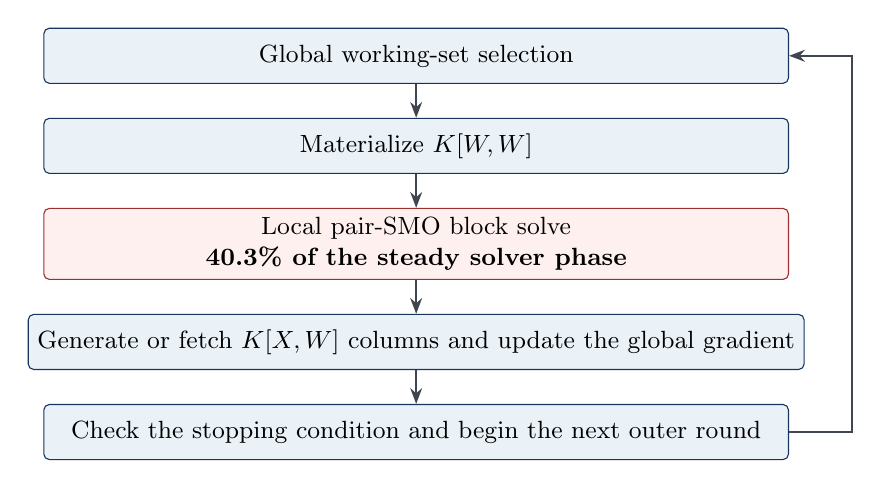
\begin{tikzpicture}[
      node distance=4.3mm,
      box/.style={draw=navy,rounded corners=2pt,fill=lightblue,
                  minimum width=0.78\textwidth,minimum height=7mm,
                  align=center,font=\small},
      hot/.style={draw=darkred,rounded corners=2pt,fill=red!6,
                  minimum width=0.78\textwidth,minimum height=7mm,
                  align=center,font=\small},
      arrow/.style={-{Stealth[length=2mm]},thick,color=darkgray}
    ]
    \node[box] (select) {Global working-set selection};
    \node[box,below=of select] (kww) {Materialize $K[W,W]$};
    \node[hot,below=of kww] (solve) {Local pair-SMO block solve\\
      \textbf{40.3\% of the steady solver phase}};
    \node[box,below=of solve] (global) {Generate or fetch $K[X,W]$ columns and update the global gradient};
    \node[box,below=of global] (stop) {Check the stopping condition and begin the next outer round};
    \draw[arrow] (select) -- (kww);
    \draw[arrow] (kww) -- (solve);
    \draw[arrow] (solve) -- (global);
    \draw[arrow] (global) -- (stop);
    \draw[arrow] (stop.east) -- ++(8mm,0) |- (select.east);
  \end{tikzpicture}
  \caption{Execution structure of the measured decomposition solver. The
  highlighted local solver becomes the dominant GPU kernel after coherent
  FP16 accelerates RBF materialization and cache traffic.}
  \label{fig:pipeline}
\end{figure}

The working-set size is typically 1,024 or 4,096. Two kernel-data units must
be distinguished:

\begin{itemize}
  \item a \emph{global column} $K[X,j]$ contains $N$ RBF values and requires
        scanning the full $N\times d$ feature matrix on a cache miss; and
  \item a \emph{local row} $K[W,j]$ contains $|W|$ values already present in
        the local $K[W,W]$ matrix and is consumed by the block solver.
\end{itemize}

They have different units and costs and must not be added as raw counts.

\subsection{Local working-set QP and serial dependence}

Define the signed working-set displacement
\begin{equation}
  s_i=y_i(\alpha_i-\alpha_i^0).
\end{equation}
The captured local problem is
\begin{equation}
  \min_{\bm{s}}
  \quad
  \bm{f}_0^{\mathsf T}\bm{s}
  +\frac{1}{2}\bm{s}^{\mathsf T}K\bm{s},
  \label{eq:local-qp}
\end{equation}
subject to
\begin{equation}
  \bm{1}^{\mathsf T}\bm{s}=0,
  \qquad
  \bm{\ell}\leq\bm{s}\leq\bm{u}.
\end{equation}
Each pair update selects an upper variable $u_t$ and a lower variable $l_t$,
computes a feasible step $q_t$, and updates the entire local gradient:
\begin{equation}
  \bm{f}^{t+1}
  =\bm{f}^{t}
  +q_t\left(K_{u_t,:}-K_{l_t,:}\right).
  \label{eq:pair-update}
\end{equation}
The next pair is selected from $\bm{f}^{t+1}$:
\begin{equation}
  (u_t,l_t)\rightarrow q_t\rightarrow \bm{f}^{t+1}
  \rightarrow (u_{t+1},l_{t+1}).
  \label{eq:serial-chain}
\end{equation}
For a valid positive-semidefinite kernel, this is a convex QP rather than an
NP-hard problem. The systems challenge is to reduce dependency depth without
increasing dense-algebra work, local-row consumption, global-column misses, or
outer rounds.

\subsection{Cost model}

We model the solver cost by three non-interchangeable terms:
\begin{equation}
  T \approx
  M_g\,C_g(N,d)
  + R_\ell\,C_\ell(|W|)
  + D\,C_d
  + T_{\mathrm{misc}},
  \label{eq:cost-model}
\end{equation}
where $M_g$ is the number of global $K[X,j]$ cache misses, $C_g$ is the cost
of producing one such column, $R_\ell$ is the number of local $K[W,j]$ row
uses, and $D$ is the number of dependent decision/update stages. A useful
optimization must reduce at least one term without causing a larger increase
in another. This model is the basis of the solver gates in
\cref{sec:boundaries}.

\section{Experimental Methodology}

\subsection{Platform and software}

\begin{table}[t]
  \centering
  \caption{Primary experimental platform.}
  \label{tab:platform}
  \begin{tabularx}{\textwidth}{@{}L{0.27\textwidth}Y@{}}
    \toprule
    Component & Configuration \\
    \midrule
    GPU & NVIDIA RTX PRO 6000 Blackwell Server Edition \\
    Target architecture & \code{sm\_120a}; driver 590.48.01 \\
    Build toolkit & CUDA 13.1 \\
    Profiled runtime & CUDA runtime 13.2 \\
    Baseline software & cuML 26.06 RBF \code{SVC.fit()} \\
    Profiling & Nsight Systems 2025.5.2 and Nsight Compute 2025.4.1 \\
    \bottomrule
  \end{tabularx}
\end{table}

Headline timings are profiler-free \code{SVC.fit()} measurements. Nsys is
used for stage attribution and NCU for selected-kernel mechanism analysis.
Final comparisons use fresh processes and balanced execution order when
available.

\subsection{Datasets and preprocessing}

\begin{table}[t]
  \centering
  \caption{Principal workloads and their role.}
  \label{tab:workloads}
  \begin{tabularx}{\textwidth}{@{}L{0.20\textwidth}L{0.25\textwidth}Y@{}}
    \toprule
    Workload & Shape & Purpose \\
    \midrule
    EMBER probe & $65{,}536\times2{,}381$ & Repeated high-dimensional timing,
      profiling, and local-solver capture \\
    EMBER full & $600{,}000\times2{,}381$ train; 200,000 test & Full-scale
      cache and low-precision gates \\
    SUSY & 4.5M train, $d=18$ & Low-dimensional scaling, row-resident reuse,
      and full KKT certification \\
    HIGGS & 10.5M train, $d=28$ & Low-dimensional full-scale generalization \\
    COD-RNA and Skin & Public low-dimensional datasets & External coverage and
      KKT certificates \\
    \bottomrule
  \end{tabularx}
\end{table}

The EMBER-65K probe is standardized with statistics computed from the probe.
The 200K held-out evaluation uses the same probe statistics because it
evaluates models trained on that probe. Full-official EMBER experiments use
statistics computed from the 600K training set. This difference is intentional
but limits direct comparison between probe and full-official campaigns.

The primary coherent-FP16 configuration uses $C=1$, $\gamma=1/2381$,
\code{tol=1e-3}, a 1,024-variable working set, and a cache capacity of 32,768
logical columns.

\subsection{Baseline and fairness dimensions}

The central performance comparison is between coherent FP16 and a
same-framework direct FP32-cache control. Both retain 32,768 logical columns;
the FP32 cache therefore consumes approximately twice the bytes of the FP16
cache. This design isolates representation and execution effects at equal
reuse capacity, not equal memory budget.

The public configuration for this comparison is
\path{artifact/configs/ember65k-ab.toml}. It names the methods
\code{direct\_fp32} and \code{coherent\_fp16}, the balanced schedule, and the
logical cache capacity without naming a machine or a particular measurement
run.

The held-out quality comparison is different: it compares the saved stock
FP32 model with the coherent-FP16 model under the same independent FP32
scorer. The performance and quality tables therefore do not share an identical
comparator. Its public experiment contract is
\path{artifact/configs/ember65k-quality.toml}, which names
\code{stock\_fp32} and \code{coherent\_fp16} and a common held-out split.

\subsection{Numerical contracts}

\paragraph{Exact-FP32 contract.}
The original FP32 RBF kernel defines the objective. Validation checks global
KKT tolerance, objective, equality feasibility, and box feasibility.

\paragraph{Coherent-low-precision contract.}
The local $K[W,W]$, global $K[X,W]$, and persistent cache consume a consistent
low-precision representation. The solver must reach its internal stopping
criterion and retain held-out predictive quality. It is not required to
reproduce every FP32 dual variable, but it must not be called an exact solution
to the original FP32 objective.

\subsection{Measurement and reporting contract}

End-to-end performance uses profiler-free fresh processes, balanced execution
order, and the complete set of repetitions rather than a selected best run.
Profiler traces are used only to attribute mechanisms and are not substituted
for end-to-end timing. Predictive quality is evaluated with a common
independent scorer, while numerical validation reports the stopping criterion
of the declared precision contract separately from an FP32-kernel audit.

Every public run emits a normalized artifact bundle. The manifest records the
configuration and source identities without machine-specific paths; the
measurement records retain method, shape, device class, solver parameters,
timing, and stopping diagnostics; and the summary contains paired statistics
and quality comparisons when requested. These machine-readable files, rather
than an opaque run name or prose log, are the unit used to compare runs.

\section{Baseline Characterization and Bottleneck Migration}

\subsection{Kernel-column reuse}

The initial exact-FP32 design targets three redundancies:

\begin{itemize}
  \item \textbf{storage:} avoid a persistent $N\times m$ dot-product or RBF
        panel when it is immediately consumed;
  \item \textbf{transfer:} fuse dot products, the RBF transform, and gradient
        accumulation to remove staging-to-cache-to-apply round trips; and
  \item \textbf{computation:} retain immutable global kernel columns in a
        bounded cache and select caching or streaming according to shape.
\end{itemize}

The full-EMBER cache-capacity sweep provides a direct mechanism result.
Increasing the FP32 cache budget from 4 GiB to 56 GiB raises hit rate from
29.6\% to 56.4\% and reduces median runtime from \SI{18.27}{s} to
\SI{13.03}{s}. This is an internal capacity effect, not a speedup over
official cuML.

\subsection{Coherent-FP16 bottleneck profile}

\begin{table}[t]
  \centering
  \caption{Nsys breakdown of the \SI{210.27}{ms} steady solver phase for
  coherent FP16 on EMBER-65K. Fractions are stage evidence, not independent
  end-to-end costs.}
  \label{tab:profile}
  \begin{tabularx}{\textwidth}{@{}Yrr@{}}
    \toprule
    Stage & Time (ms) & Fraction \\
    \midrule
    \code{SmoBlockSolveCoarsened} & 84.75 & \textbf{40.3\%} \\
    Full-data FP16 cache-miss materializer & 44.55 & 21.2\% \\
    Coherent FP16 $K[W,W]$ materializer & 7.41 & 3.5\% \\
    FP16 cached-column apply & 8.79 & 4.2\% \\
    Remaining GPU work & 15.87 & 7.5\% \\
    Launch, synchronization, and host gaps & 48.90 & 23.3\% \\
    \bottomrule
  \end{tabularx}
\end{table}

NCU shows that the block solver launches one 256-thread CTA and reaches only
0.11\% whole-device SM throughput and 0.17\% DRAM throughput. PC sampling is
dominated by wait, scoreboard, and barrier stalls. This does not prove that a
parallel replacement will be faster. It identifies a dependency-limited
kernel rather than an FP16 throughput bottleneck.

The full-data materializer has two regimes. Large panels achieve higher
compute throughput, whereas small panels scan the full feature matrix and are
predominantly DRAM-bound. The implementation dispatches 32,000 padded columns
for 20,114 useful new columns. Removing padding is useful, but a full-$X$ scan
sets a floor that prevents a linear conversion of padded work into wall-time
savings.

\section{Dataflow and Precision Mechanisms}

\subsection{Coherent FP16}

A naive half-cache path stores RBF values in FP16 while constructing the local
$K[W,W]$ in FP32. The optimizer then consumes two inconsistent versions of
the same kernel. On EMBER-65K, this design requires 192 outer rounds, compared
with 152 for the direct FP32-cache control.

The coherent-FP16 path instead enforces the following execution invariant:
all decision-relevant local and global kernel values derive from the same
quantized inputs and distance rules. The implementation uses half precision
for training features or persistent RBF values, Tensor Cores for
high-dimensional dot-product tiles, and FP32 for the RBF transform,
accumulation, dual variables, gradients, and SMO control. It also avoids a
large FP32 staging panel.

With coherent values, outer rounds fall to 146. The mechanism is therefore not
simply that FP16 arithmetic is faster. A stateful optimizer must see one
coherent approximate operator at every point where it makes decisions.

\subsection{Shape-aware low-dimensional reuse}

The general high-dimensional TMA path pads SUSY from $d=18$ to $d=64$. The
compact path stores the original 18 features, uses aligned \code{half2} loads,
keeps two adjacent training rows per thread, stages 32 working-set rows at a
time, and accumulates RBF and gradient updates in FP32.

Relative to the strongest reuse-aware FP32 baseline, compact coherent FP16
improves SUSY-65K by 1.0995$\times$ and SUSY-1M by 1.0958$\times$. The generic
padded path is approximately neutral or slower. Low- and high-dimensional
workloads therefore require different kernels: Tensor Core dot products are
valuable in high dimensions, while eliminating padding and repeated row loads
matters more in low dimensions.

\subsection{Decision-path-aware block-solver micro-optimization}

The local solver repeatedly scans candidates, ranks lower variables, computes
an accepted step, and identifies threads that own selected variables. The
accepted micro-optimization uses approximate division only for broad
candidate ranking, retains exact FP32 arithmetic for the committed step $q$,
and replaces an all-thread owner search with direct index mapping.

Across eight captured snapshots, the candidate reproduces the captured
trajectory. In the formal end-to-end run, however, iteration counts differ
slightly (46,854 versus 46,861) and one of 65,536 training predictions differs.
The defensible description is therefore \emph{snapshot-equivalent and
quality-equivalent under the coherent-FP16 contract}, not globally
bitwise-exact.

\subsection{Lower precision beyond FP16}

Lower bit widths do not automatically extend the FP16 result.

\begin{itemize}
  \item An MXFP8-compute path with an FP16 cache retains much of the measured
        quality but does not establish a uniformly stronger mechanism.
  \item A linear U8 RBF cache doubles cache-column capacity and reduces one
        full-EMBER fit from \SI{4.865}{s} to \SI{3.734}{s}
        (1.303$\times$), but test accuracy falls from 0.92648 to 0.75329.
  \item An NVFP4 reconstructed-input gate reaches the internal tolerance and
        changes EMBER-65K training accuracy by $-3.05\times10^{-5}$. Its
        fit-time ratio is approximately 1.007$\times$ and preprocessing is
        excluded; the SVM kernel is not executed natively in FP4.
\end{itemize}

Feature quantization, RBF exponentiation, cache encoding, local
materialization, and solver state must form one coherent data path. Peak FP8
or FP4 GEMM throughput alone is not an end-to-end argument.

\section{Evaluation of Positive Mechanisms}

\subsection{Matched coherent-FP16 performance}

\begin{table}[t]
  \centering
  \caption{Seven-run EMBER-65K comparison using fresh processes and balanced
  order. The direct FP32 and coherent-FP16 controls have equal logical
  cache-column capacity (32,768), not equal cache bytes.}
  \label{tab:coherent-performance}
  \begin{tabularx}{\textwidth}{@{}Yrrrr@{}}
    \toprule
    Method & Median fit (s) & CV & Outer rounds & Accuracy \\
    \midrule
    Direct slotted FP32 cache & 0.486954 & 3.60\% & 152 & 0.957321 \\
    FP16 cache, FP32 $K[W,W]$ & 0.530813 & 2.60\% & 192 & 0.957153 \\
    Coherent FP16 & \textbf{0.360385} & 4.05\% & 146 & 0.957123 \\
    \bottomrule
  \end{tabularx}
\end{table}

Coherent FP16 is 1.351$\times$ faster than the direct FP32-cache control, with
a 95\% bootstrap confidence interval of
1.263$\times$--1.403$\times$. The incoherent half-cache path is slower despite
lower storage precision because its outer-round count increases by 26.3\%.

\subsection{Held-out predictive quality}

\begin{table}[t]
  \centering
  \caption{Independent FP32 scoring on all 200,000 official EMBER test
  samples. This comparison uses the saved stock FP32 and coherent-FP16 models;
  it is not the same baseline pair as \cref{tab:coherent-performance}.}
  \label{tab:quality}
  \begin{tabularx}{\textwidth}{@{}Yrrr@{}}
    \toprule
    Metric & Stock FP32 & Coherent FP16 & Difference \\
    \midrule
    Accuracy & 0.830980 & 0.830895 & $-0.000085$ \\
    ROC AUC & 0.93525055 & 0.93516107 & $-0.00008948$ \\
    TPR at 0.1\% FPR & 0.28222 & 0.28084 & $-0.00138$ \\
    TPR at 1\% FPR & 0.48384 & 0.48316 & $-0.00068$ \\
    \bottomrule
  \end{tabularx}
\end{table}

The models disagree on 179 of 200,000 predictions. Stock is uniquely correct
on 98 examples and coherent FP16 on 81. The exact McNemar $p$-value is
0.231645, and decision scores have Pearson correlation 0.9999813. The result
means that this experiment did not detect a statistically significant
accuracy difference; it is not an equivalence test with a predeclared margin.

The coherent solver satisfies its own final gap,
$9.97663\times10^{-4}$, at a tolerance of $10^{-3}$. Under an independently
reconstructed original FP32 kernel, however, the maximum KKT residual is
0.058432, with 4,847 samples above $10^{-3}$. A sampled
1,024-by-1,024 FP16-rounded RBF matrix is mildly indefinite, with minimum
eigenvalue $-0.00413$. The artifact must not be called an exact FP32
replacement or a proven convex SVM for a newly defined kernel.

\subsection{Block-solver micro result}

The decision-path-aware micro-optimization accelerates the isolated block
solver by 1.096$\times$--1.106$\times$. In a provenance-complete,
direction-balanced 11-pair campaign, median fit time falls from 0.359733 s to
0.348284 s. The median-ratio speedup is 1.0329$\times$, the paired
geometric-mean speedup is 1.0376$\times$, and the paired bootstrap 95\%
interval is 1.0050$\times$--1.0708$\times$. It wins 8 of 11 pairs.

This experiment supports a numerical asymmetry: approximation can be safe for
broad candidate ranking while remaining unsafe for the committed state
transition. It is a useful retained optimization, but its magnitude is
insufficient as a standalone solver contribution.

\section{Empirical Design-Space Boundaries}
\label{sec:boundaries}

\subsection{Work-depth objective}

For a local solve, define $D$ as the number of dependent decision/update
stages and $R_\ell$ as the number of local kernel-row uses. A useful GPU solver
must reduce $D$ without causing an offsetting increase in $R_\ell$, global
column misses $M_g$, or outer rounds.

An oracle experiment supplies the exact $(u_t,l_t)$ sequence and removes pair
selection. The residual exact step and 1,024-element update still require
1,456.77 cycles per committed step, compared with 3,789.52 cycles for the
baseline. Perfect pair prediction provides a 2.60$\times$ isolated upper
bound, but already exceeds the predeclared 1,200-cycle floor before prediction,
validation, rollback, or contention. Pair selection is expensive, but it is
not the entire bottleneck.

\subsection{Rejected hypotheses}

\footnotesize
\begin{longtable}{@{}L{0.21\textwidth}L{0.36\textwidth}L{0.35\textwidth}@{}}
  \caption{Decision-relevant empirical boundaries for block-solver redesign.}
  \label{tab:nogo}\\
  \toprule
  Hypothesis & Minimal experiment and result & Causal explanation \\
  \midrule
  \endfirsthead
  \multicolumn{3}{l}{\small\itshape Table~\thetable\ continued}\\
  \toprule
  Hypothesis & Minimal experiment and result & Causal explanation \\
  \midrule
  \endhead
  \midrule
  \multicolumn{3}{r}{\small\itshape Continued on the next page}\\
  \endfoot
  \bottomrule
  \endlastfoot

  Whole-working-set projected or Newton solve &
  Eight real $1{,}024^2$ EMBER subproblems. Retained-set SMO passes 7/8 cases
  in 11--24 phases but is 6.52$\times$ slower in CUDA. Semismooth Newton passes
  8/8 but requires 87--164 dense solves; one Newton solve per phase fails early
  and middle snapshots. &
  Counting outer phases hides the dependent linear-solve depth. Free sets
  become large, matrices are ill-conditioned, and small dense solves are not
  cheap relative to optimized SMO. \\

  Fixed-depth joint block QP &
  PN1-B8 is correct on 10/10 snapshots. Median conservative depth reduction is
  1.84$\times$ on SUSY and 2.24$\times$ on EMBER. Integrated CUDA is
  5.56$\times$--7.15$\times$ slower and reduces outer scans only from 34 to 32. &
  The eight pairs are still constructed sequentially and each joint update
  streams up to 16 local rows. Algebraic batching does not reduce row work or
  outer full-data scans. \\

  Sampled lower-variable selection &
  Random and sampled-best candidate sets reduce per-step selection work but
  require more pair and outer updates at the same stopping target. &
  Candidate quality falls faster than selection cost; a cheaper step is not
  useful when more steps and kernel data are required. \\

  Scan/update fusion and ratio rewrites &
  Scan/update fusion preserves snapshot output but runs at
  0.73--0.78$\times$ baseline speed. Cross-multiplied ratio ranking runs at
  0.87--0.93$\times$. Fast $q$ changes trajectories and regresses end-to-end
  time. &
  Fusion extends the live dependency chain and increases instruction or
  register pressure. Approximation is unsafe on the committed step even when
  acceptable for ranking. \\

  Geometry-aware packing and GraphSMO &
  Offline geometry is promising, but real SUSY replay yields a
  0.99$\times$ unique-local-endpoint ratio and a 1.00$\times$ net-committed
  endpoint ratio relative to a strong geometry-block control. &
  The local path changes, but the set of expensive rows does not shrink.
  Control-batch reduction alone is insufficient. \\

  Temporal tiling &
  The best oracle configuration converges in a median 12.5 phases but retains
  a 0.966 median propagated-column ratio. Local endpoint reuse is only 2.74\%. &
  Local state is already register-resident, and successive pair updates rarely
  reuse or cancel endpoints. Deferring propagation groups barriers without
  removing work. \\

  Stale top-16 SpecSMO &
  Stale top-16 coverage reaches 84.22\%, but a zero-overhead supplied-$u$
  oracle has only a 1.226$\times$ optimistic upper bound. &
  Candidate stability is real, yet lower-variable selection, exact $q$, and
  the local-state update dominate after $u$ is supplied. \\

  Exact full-pair replay &
  Across 2,896 bitwise-checked steps, supplying $(u,l)$ reduces cost from
  3,789.52 to 1,456.77 cycles per step but fails the 1,200-cycle gate. &
  The residual exact step, two local-row reads, and 1,024-element state update
  form a substantial serial floor. \\

  Triangular pair batching &
  The recurrence is numerically valid, but 32.6\% of steps hit box bounds.
  Chunk 32 achieves only 2.386$\times$ depth reduction and
  1.005$\times$ local-row byte reduction. &
  Box clipping terminates the recurrence, and the exact pair stream has almost
  no endpoint reuse. TRSV changes algebraic form, not trace structure. \\

  Bounded speculative prefetch &
  Six direction-balanced full-EMBER pairs increase median fit time from
  4.8746 s to 5.2213 s. The path avoids 6,884 demand misses but generates
  15,744 speculative global columns. &
  The current working set is an inaccurate predictor of future cache columns.
  Apparent overlap is purchased with additional materialization and resource
  contention. \\
\end{longtable}
\normalsize

\subsection{Gate for a future solver}

A new mechanism should proceed to a full CUDA implementation only if one fixed
configuration satisfies the following conditions on real early-, middle-, and
late-training subproblems:

\begin{enumerate}
  \item preserve box and equality feasibility, captured objective progress,
        and the local stopping contract;
  \item reduce conservative dependency depth by at least 4$\times$;
  \item keep net committed local-row endpoints below 1.25$\times$ the pairwise
        baseline, preferably reducing them;
  \item generate all joint directions in a bounded number of full-working-set
        passes rather than hiding serial pair construction inside a block;
  \item include online direction generation, validation, fallback, and
        rollback rather than relying on an oracle trace;
  \item reach at most 1,200 cycles per committed-equivalent update or at least
        2$\times$ isolated block-solver speedup;
  \item avoid increasing global-column misses or outer full-data scans; and
  \item pass direction-balanced, profiler-free end-to-end training under the
        same numerical contract.
\end{enumerate}

\section{Open-Source Artifact and Transferable Mechanism}
\label{sec:artifact}

The public artifact is organized as a fresh repository named
\code{coherent-svm}. It is not a snapshot of the development tree. The
release contains only the code, configurations, schemas, and documentation
needed to explain and validate the transferable mechanism: one rounded kernel
operator must be used consistently by materialization, caching, local
decisions, and global updates.

\noindent Public repository:
\url{https://github.com/yongqiu-star/coherent-svm}.

\subsection{Mechanism interface}

The central invariant can be expressed independently of a particular GPU
microkernel. Let $Q_p(X_i,X_j)$ denote the declared represented kernel,
including input conversion, dot-product precision, distance rules, and cache
encoding. The same $Q_p$ is used at every state-changing boundary:

\begin{lstlisting}[style=codeblock]
for each outer working set W:
    Kww = materialize(X[W], X[W], operator=Qp)
    delta_alpha = solve_local_qp(Kww, state, representation=Qp)

    for each required global column j in W:
        if cache.contains(j):
            column = cache.load(j)              # already in Qp
        else:
            column = materialize(X, X[j], operator=Qp)
            cache.insert(j, column)
        global_gradient += column * delta_alpha[j]

    select_next_working_set(global_gradient, representation=Qp)
\end{lstlisting}

The key invariant is operator identity: a cache hit, a newly produced column,
the local Hessian, and the gradient update all observe values generated by
the same $Q_p$. Mixed-precision accumulation and scalar control are permitted;
silently changing the kernel operator between producers and consumers is not.

\subsection{Portable reference backend}

The public repository provides a portable CUDA C++ and cuBLAS reference
backend. It uses documented APIs rather than architecture-specific inline
PTX. The release is deliberately small: the backend is in
\path{src/portable_fp16_rbf_backend.cu}; the cuML integration is a versioned
patch; \path{coherent_svm/} contains the runner and provenance code; and
\path{artifact/configs/} contains the experiment contracts. This backend is
intended to validate:

\begin{itemize}
  \item representation coherence across the full state transition;
  \item cache hit/miss semantics and equal-logical-capacity comparisons;
  \item integration of materialization, local solve, and global update; and
  \item normalized timing and held-out-quality outputs.
\end{itemize}

The reference backend is not claimed to reproduce the reported
1.351$\times$ speedup. That result was measured with an aggressively optimized
\code{sm\_120a} backend whose development tree still contains
third-party-derived components without complete file-level redistribution
provenance. Publishing that backend before provenance and license boundaries
are resolved would be misleading. It is therefore excluded from the public
release. The measured performance claim and the portable mechanism artifact
are deliberately reported as two different scopes.

\subsection{Public configurations and normalized manifests}

Stable public configuration identifiers describe the experiment without
encoding a host, user, or private workspace. The central files are listed in
\cref{app:public-configs}. Each run records:

\begin{itemize}
  \item a manifest with the configuration digest, public source revision,
        library digest, logical dataset identifier, and platform class;
  \item per-process measurements with method, shape, device class, solver
        parameters, fit status, iterations, support-vector count, and timing;
  \item summary statistics and explicit completion/finite-value checks; and
  \item for the held-out configuration, accuracy, AUC, prediction
        disagreements, McNemar's exact test, and score correlation.
\end{itemize}

This schema makes the artifact useful even on hardware that cannot reproduce
the optimized backend: the semantic contract and the experiment denominator
remain inspectable and comparable.

The public runner does not automate the independent FP32-objective KKT audit
used in the report. That audit remains a model-difference diagnostic rather
than the convergence definition of the coherent low-precision solver.

\subsection{Transferable lesson}

The artifact treats coherent low precision as an algorithm--system interface,
not as an isolated datatype substitution. The same pattern applies to other
iterative GPU algorithms when cached or materialized values influence future
control decisions: define the approximate operator, make every state-changing
consumer agree on it, and then optimize storage and compute within that
contract. Peak throughput is secondary to preserving a productive and
well-defined state trajectory.

\section{Discussion and Design Implications}

\subsection{Coherence before precision}

Low precision changes an iterative solver in two ways. It changes arithmetic
values, and it can change the decisions made from those values. In pair-SMO,
a small perturbation can select a different pair; that pair changes the next
gradient, which changes every subsequent selection. Precision is consequently
not a local property of the GEMM that produces a dot product or of the cache
that stores an RBF value. It is a property of the induced state-transition
system.

This explains why converting only the cache can be both smaller and slower.
If the local solver selects pairs using one representation while the global
gradient is updated with another, the implementation repeatedly reconciles
two different operators and may follow a less productive trajectory. Coherent
FP16 succeeds by making the materializer, cache, and decision-making consumers
agree on the same rounded kernel. It does not require every scalar control
operation to use FP16. The transferable rule is therefore
\emph{coherence before precision}: first define which approximate operator the
algorithm solves, then choose the precision of each operation while preserving
that operator at every state-changing boundary.

\subsection{Progress per kernel-data item}

The conventional metrics for a GPU kernel---throughput, occupancy, bytes per
second, or pair updates per second---do not measure whether an optimization
solver is moving efficiently toward its target. In this workload, a global
column $K[X,j]$ may require a full $N\times d$ feature scan, whereas a local
row $K[W,j]$ is read from an already materialized working-set matrix. Counting
both as one ``kernel row'' obscures the dominant cost.

A more useful comparison couples the weighted work in
\cref{eq:cost-model} with optimization progress. For example, over an interval
$[t,t+r]$, one can report
\begin{equation}
  \eta_{\mathrm{kernel}}
  =
  \frac{\Phi(\bm{\alpha}^{t})-\Phi(\bm{\alpha}^{t+r})}
       {M_g C_g(N,d)+R_\ell C_\ell(|W|)},
  \label{eq:progress-per-kernel-data}
\end{equation}
where $\Phi$ is the minimized dual objective and the denominator weights
global-column generation separately from local-row use. KKT-gap reduction can
be substituted when objective values are unavailable. This metric exposes a
common failure mode: a speculative method can execute more GPU work per
second while obtaining less progress from every generated column.

The resulting design goal is not simply to maximize cache hits or reduce pair
latency. It is to reuse every expensive, immutable kernel column for enough
useful local progress to amortize its generation, without over-solving a stale
working set. This framing applies more broadly to iterative GPU algorithms in
which expensive data products feed a sequence of state-dependent decisions.

\subsection{Work--depth, not occupancy}

The serial chain in \cref{eq:serial-chain} creates low device utilization, but
launching more work does not remove the dependence. Large-block methods,
fixed-depth replay, and speculative prefetch can expose more parallelism while
also introducing larger Hessians, additional local rows, wasted global
columns, projection work, or extra outer rounds. Occupancy improves even when
time to convergence does not.

The relevant abstraction is a work--depth frontier. Here, work includes the
first two terms of \cref{eq:cost-model}, while depth counts state-changing
decision stages that cannot overlap. A useful parallel solver must reduce
depth faster than it increases weighted kernel-data work. The fixed-depth and
triangular experiments fail this test: they shorten or regularize control but
leave too much row work unchanged. This is a stronger conclusion than
``the GPU is underutilized.'' It identifies what a replacement algorithm must
change: the optimization directions themselves must yield more progress per
dependent stage.

\subsection{Shape and phase are first-class inputs}

The profitable execution regime is nonuniform in both data shape and solver
state. At $d=18$ or 28, padding, repeated local-row loads, and solver control
can dominate because each kernel evaluation contains little arithmetic. At
$d=2{,}381$, Tensor Core dot products, full-data column misses, cache capacity,
and the local solver are all material. A representation or tiling strategy
that is effective in one regime can add overhead in the other.

The same nonuniformity appears over time. In the measured exact trace, late
outer rounds 100--140 contain residual-limited runs with a local
5$\times$--7$\times$ depth opportunity, whereas early and middle rounds are
frequently interrupted by box constraints. This suggests phase-aware solver
selection, but it does not make adaptation free: each phase-specific primitive
must first be profitable on its own, and the switching signal must cost less
than the work it avoids.

Taken together, these results favor dispatch over a universal kernel. Feature
dimension, working-set size, cache state, active constraints, and recent
progress should select among mechanisms only when each mechanism has a
measured region of advantage.

\subsection{Amdahl limits and co-design priorities}

The steady solver phase in \cref{tab:profile} makes the remaining limits
concrete. Completely deleting the 44.55 ms materializer would provide at most
approximately 1.27$\times$ speedup. Completely deleting the 84.75 ms block
solver would provide at most approximately 1.68$\times$. A realistic
2$\times$ improvement in only one stage yields approximately 1.12$\times$ and
1.25$\times$, respectively. Thus, no remaining microkernel alone can deliver
a 2$\times$ end-to-end gain on this workload.

The more promising target is an algorithm--system co-design that changes both
terms: use a representation that increases reuse and lowers column cost, then
use a solver that obtains more progress before the next full-data update. Such
a design should be judged by three questions: how many new global columns it
generates, how many local rows it consumes, and how much objective or KKT
progress it obtains before the next dependent decision. These questions turn
the present negative results into reusable gates for future designs rather
than implementation-specific anecdotes.

\section{Related Work}

SMO reduces an SVM dual problem to analytically solvable two-variable updates
\cite{platt1999smo}. Second-order working-set selection, as used by LIBSVM and
related decomposition solvers, trades additional candidate scoring for fewer
optimization steps~\cite{fan2005working,chang2011libsvm}. This tradeoff is
directly visible in our sampled-candidate experiments: cheaper selection
increases the number of committed updates.

GPU SVM systems have long accelerated kernel evaluation and solver updates.
Catanzaro et al.\ demonstrated early GPU-oriented training and classification
\cite{catanzaro2008gpu}, while ThunderSVM provides a later GPU/CPU SVM
implementation with an optimized working-set pipeline~\cite{wenthundersvm}.
The current study differs in emphasis. It begins from cuML's production RBF
solver, separates global column generation from local-row consumption, and
uses exact GPU traces to measure the residual work after pair selection is
removed.

Block decomposition, active-set, and Newton methods are established approaches
to convex QP optimization. Our contribution is not a new general convergence
theory. It is an empirical systems boundary on the captured GPU subproblems:
free sets become large, dense solves remain dependent, and algebraic batching
does not reduce enough kernel-row work to beat an optimized pair-SMO kernel.

\section{Threats to Validity and Limitations}

\paragraph{Workload coverage.}
The decision-grade coherent-FP16 result is concentrated on EMBER-65K with one
hyperparameter setting. SUSY and HIGGS provide shape diversity, but their
largest speedups are historical screening evidence rather than matched
official-baseline results.

\paragraph{Fairness dimensions.}
The 1.351$\times$ comparison fixes logical cache capacity, not bytes. This is
appropriate for studying representation and reuse but gives FP16 a smaller
memory footprint. The 2.371$\times$ stock comparison is explicitly contextual
because cache budgets differ substantially.

\paragraph{Quality inference.}
A non-significant McNemar result is not proof of equivalence. No equivalence
margin was predeclared, and cross-dataset quality is not established. The
reported AUC and tail metrics also change slightly.

\paragraph{Numerical objective.}
Coherent FP16 passes its internal stopping criterion but not the original
FP32-kernel KKT audit. A sampled rounded RBF matrix is mildly indefinite.
Claims are therefore limited to measured predictive quality and the declared
low-precision execution contract.

\paragraph{Preprocessing.}
The EMBER probe and full-official campaigns use different training statistics.
The 200K test set is standardized with probe statistics only when evaluating
probe-trained models.

\paragraph{Profiling and capture.}
Nsys and NCU perturb timing and are used only for attribution. One early
real-working-set capture lacked a complete source-to-binary chain; later clean
GPU traces validate final alpha and delta behavior. A publication artifact
should nevertheless recapture every central snapshot from one released tree.

\paragraph{Hardware scope.}
The primary target is one RTX PRO 6000 Blackwell GPU. The conclusions may
change with memory capacity, Tensor Core ratios, or launch characteristics on
other architectures. Multi-GPU experiments did not establish a stable
convergence contract and are excluded from the main analysis.

\section{Conclusion}

This study shows that accelerating nonlinear GPU SVM training requires more
than a faster RBF kernel. Kernel-column reuse, fused dataflow, and a coherent
FP16 operator reduce redundant computation and memory traffic, producing a
1.351$\times$ matched speedup on EMBER-65K. A separate held-out evaluation
detects no statistically significant accuracy difference in the measured
experiment. The numerical solution nevertheless differs from the original
FP32-kernel objective, so the result is a useful low-precision execution
contract rather than an exact FP32 replacement.

The optimized pipeline reveals a more general systems lesson. Once regular
numeric work becomes inexpensive, the limiting resource can become dependent
optimization progress. The local pair-SMO solver does not lack arithmetic
throughput; each accepted step determines the next decision. Attempts to fill
the GPU by batching, replaying, or speculating can reduce visible depth while
increasing global-column generation, local-row consumption, or outer
iterations. Their success must therefore be measured by progress per weighted
kernel-data item, not occupancy alone.

Four principles emerge: preserve one coherent approximate operator across all
state-changing components; distinguish expensive global data production from
local data reuse; optimize the work--depth frontier rather than either axis in
isolation; and treat workload shape and solver phase as first-class dispatch
inputs. These principles are not specific to SVMs. They apply whenever an
iterative GPU algorithm alternates high-throughput data production with a
short, state-dependent decision chain. For RBF SVMs, the remaining opportunity
is a solver that discovers several jointly productive directions from each
working set, thereby obtaining substantially more convergence progress from
every generated kernel column without sacrificing the declared numerical
contract.

\appendix

\section{Claim-to-Public-Artifact Matrix}
\label{app:public-configs}

\begin{table}[H]
  \centering
  \caption{Public files associated with the report's central claims.}
  \begin{tabularx}{\textwidth}{@{}L{0.22\textwidth}L{0.30\textwidth}Y@{}}
    \toprule
    Purpose & Public artifact & Reproducibility boundary \\
    \midrule
    Portable numerical correctness &
      \path{tests/test_portable_backend_gpu.py} and
      \path{artifact/configs/smoke-synthetic.toml} &
      Compares FP32 and FP16 cache materialization and the full
      $K\Delta\alpha$ update with an explicit RBF oracle; also exercises the
      patched solver end to end. \\
    Matched performance protocol &
      \path{artifact/configs/ember65k-ab.toml} and
      \path{artifact/reference/pro6000.json} &
      Encodes equal logical cache capacity and balanced repetitions. The
      public portable backend does not reproduce the 1.351$\times$
      architecture-tuned result. \\
    Held-out quality protocol &
      \path{artifact/configs/ember65k-quality.toml} &
      Runs stock FP32 and coherent FP16 on one held-out split and summarizes
      accuracy, AUC, disagreements, McNemar's exact test, and score
      correlation. It is not an equivalence proof. \\
    Work--depth analysis &
      \path{studies/work-depth/metrics.py} &
      Separates global columns, local rows, and dependent decision stages.
      The private captured traces used in the report are not redistributed. \\
    \bottomrule
  \end{tabularx}
\end{table}

The source release is intentionally smaller than the development workspace.
Generated datasets, binaries, profiler reports, and failed experimental
branches are not required to understand or exercise the mechanism.

\section{Repository Layout and Quick Start}
\label{app:quick-start}

The fresh public repository has the following stable surface:

\begin{lstlisting}[style=codeblock]
coherent-svm/
|-- src/portable_fp16_rbf_backend.cu
|-- include/
|-- patches/cuml-26.06.00/
|-- coherent_svm/
|-- artifact/configs/
|-- artifact/schemas/
|-- studies/work-depth/
`-- tests/
\end{lstlisting}

The repository is public; only dependency paths remain machine-specific:

\begin{lstlisting}[style=codeblock]
git clone https://github.com/yongqiu-star/coherent-svm
cd coherent-svm
uv sync --frozen --extra gpu --extra quality --extra dev
uv run coherent-svm doctor

export CUML_SOURCE=<path-to-cuml-26.06.00>
export CUVS_INCLUDE=<path-to-cuvs-include>
git -C "$CUML_SOURCE" apply \
  "$PWD/patches/cuml-26.06.00/coherent-fp16.patch"
PYTHON="$PWD/.venv/bin/python" scripts/build.sh

COHERENT_SVM_LIBRARY=build/libcoherent_svm.so \
  uv run pytest -q
uv run coherent-svm reproduce \
  --config artifact/configs/smoke-synthetic.toml \
  --library build/libcoherent_svm.so \
  --output-root results
\end{lstlisting}

The main prepared-data protocol replaces the smoke configuration with
\path{artifact/configs/ember65k-ab.toml} and adds
\code{--data-root <prepared-data-root>}. Dataset arrays remain external to the
repository; their normalized layout is documented in
\path{artifact/README.md}. The release specifies the prepared-array contract
but does not include EMBER's feature-extraction pipeline.
The complete patched-solver reproduction path currently requires compute
capability 12.0; the standalone portable-backend oracle test builds for the
local CUDA architecture.

\section{Normalized Output Contract}
\label{app:output-contract}

Each reproduction writes five public files:

\begin{lstlisting}[style=codeblock]
results/<config-id>/<run-id>/
|-- manifest.json
|-- measurements.jsonl
|-- summary.json
|-- checks.json
`-- artifacts.sha256
\end{lstlisting}

The manifest retains the public source revision, dirty state, configuration
and library digests, logical dataset identifier, Python version, and platform
class. It intentionally omits the hostname, user name, GPU UUID, private Git
remote, and absolute command paths. Shape, device model, compute capability,
solver parameters, timing, iteration count, and sampled training accuracy are
written with each measurement rather than hidden in a prose log.

For example, the balanced performance summary has the following stable
shape; absolute times are observations rather than cross-machine pass
conditions:

\begin{lstlisting}[style=codeblock]
{
  "config_id": "ember65k-ab",
  "baseline": {"method": "direct_fp32",
               "median_fit_seconds": "<measured>"},
  "candidate": {"method": "coherent_fp16",
                "median_fit_seconds": "<measured>"},
  "speedup": "<ratio>",
  "speedup_ci95": ["<low>", "<high>"],
  "repeats": 7
}
\end{lstlisting}

\section{Licensing and Redistribution Boundary}
\label{app:licensing}

The original reference backend, runner, configurations, schemas, tests, and
documentation are released under Apache-2.0. Changes to cuML are distributed
as patches against cuML 26.06.00 and retain the upstream license notices when
applied. CUDA, cuBLAS, cuML, RAPIDS dependencies, and datasets are external;
the repository neither vendors their binaries nor redistributes raw data.

The optimized \code{sm\_120a} backend is excluded because file-level
provenance and redistribution rights for all third-party-derived components
have not yet been resolved. This is a release boundary, not a performance
claim: the portable backend validates the coherent operator and integration,
whereas the 1.351$\times$ measurement describes the unreleased tuned backend.
A later release of that backend requires an independent provenance and
licensing review.

\begin{thebibliography}{9}

\bibitem{platt1999smo}
J. C. Platt.
\newblock Fast training of support vector machines using sequential minimal
optimization.
\newblock In B. Sch\"olkopf, C. J. C. Burges, and A. J. Smola, editors,
\emph{Advances in Kernel Methods: Support Vector Learning}, pages 185--208.
MIT Press, 1999.

\bibitem{fan2005working}
R.-E. Fan, P.-H. Chen, and C.-J. Lin.
\newblock Working set selection using second order information for training
support vector machines.
\newblock \emph{Journal of Machine Learning Research}, 6:1889--1918, 2005.

\bibitem{chang2011libsvm}
C.-C. Chang and C.-J. Lin.
\newblock LIBSVM: A library for support vector machines.
\newblock \emph{ACM Transactions on Intelligent Systems and Technology},
2(3):27:1--27:27, 2011.

\bibitem{catanzaro2008gpu}
B. Catanzaro, N. Sundaram, and K. Keutzer.
\newblock Fast support vector machine training and classification on graphics
processors.
\newblock In \emph{Proceedings of the 25th International Conference on Machine
Learning}, pages 104--111, 2008.

\bibitem{wenthundersvm}
Z. Wen, J. Shi, B. He, J. Chen, K. Li, and X. Chen.
\newblock ThunderSVM: A fast SVM library on GPUs and CPUs.
\newblock \emph{Journal of Machine Learning Research}, 19(21):1--5, 2018.

\end{thebibliography}


\end{document}
